\documentclass[UTF8,a4paper,12pt]{ctexbook} 

 \usepackage{graphicx}%学习插入图
 \usepackage{verbatim}%学习注释多行
 \usepackage{booktabs}%表格
 \usepackage{geometry}%图片
 \usepackage{amsmath}
 \usepackage{amssymb}
 \usepackage{listings}%代码
 \usepackage{xcolor}  %颜色
 \usepackage{enumitem}%列表格式
 \usepackage{algorithm}  %format of the algorithm
 \usepackage{algorithmic}%format of the algorithm
 \usepackage{multirow}   %multirow for format of table
 \usepackage{hyperref} %超链接 \url{URL}
  \usepackage{tabularx} 	%表格排版格式控制
  \usepackage{array}	%表格排版格式控制
 \CTEXsetup[format+={\flushleft}]{section}
 
 \newcommand{\EQ}[1]{$\textbf{EQ:}#1\ $}
 \newcommand{\ALGORITHM}[1]{$\textbf{Algorithm:}#1\ $}
 \newcommand{\Figure}[1]{$\textbf{Figure }#1\ $}
 \renewcommand{\figurename}{Fig}
 
 \graphicspath{{figure/}}
 \geometry{left=1.6cm,right=1.8cm,top=2cm,bottom=1.7cm} %设置文章宽度

  %代码效果定义
  \definecolor{mygreen}{rgb}{0,0.6,0}
  \definecolor{mygray}{rgb}{0.5,0.5,0.5}
  \definecolor{mymauve}{rgb}{0.58,0,0.82}
  \lstset{ %
  	backgroundcolor=\color{white},   % choose the background color
  	basicstyle=\footnotesize\ttfamily,        % size of fonts used for the code
  	columns=fullflexible,
  	breaklines=true,                 % automatic line breaking only at whitespace
  	captionpos=b,                    % sets the caption-position to bottom
  	tabsize=4,
  	commentstyle=\color{mygreen},    % comment style
  	escapeinside={\%*}{*)},          % if you want to add LaTeX within your code
  	keywordstyle=\color{blue},       % keyword style
  	stringstyle=\color{mymauve}\ttfamily,     % string literal style
  	frame=single,					%tb top and bottom; L left double line
  	xleftmargin=.06\textwidth, 
  	%xrightmargin=.1\textwidth,
  	rulesepcolor=\color{red!20!green!20!blue!20},
  	% identifierstyle=\color{red},
  	language=c++,
  }
%设置页面布局
\pagestyle{plain}
\author{\kaishu 郑华}
\title{\textbf{C++\_STL 总结}}

 %正文排版开始
 \begin{document} 
 	\maketitle
 	
 	\tableofcontents


		
		
		
\chapter{容器-Container}
\section{容器底层数据结构实现}
	\subsection{总结}
		 \paragraph{0.tuple}    tuple元组是一个固定大小的不同类型值的集合,可以用来代替简单的结构体
			 \begin{lstlisting}
	#include <tuple>
	#include <string>
	#include <iostream>
	using namespace std;
	int main(int arc,char** argv)
	{
		using MyTuple = tuple < int, string > ;
		
		tuple < int, string > tup1 = make_tuple(1, "jack");	// 创建一个MyTuple类型的元组
		MyTuple tup2 = make_tuple(2, "lily");	// 创建一个MyTuple类型的元组
		
		int var = 3;
		auto tup3 = tie(var,tup1,tup2);				// 创建一个tuple < int, MyTuple, MyTuple>类型的元组
		
		cout << get<0>(tup1) << endl;			// 输出 1
		cout << get<1>(tup2) << endl;			// 输出 lily
		cout << get<1>(get<1>(tup3)) << endl; // 输出 jack
		
		return 0;
	}
			 \end{lstlisting}
			 
		 \paragraph{1.vector}      底层数据结构为\textbf{数组} ,支持快速随机访问
			 \subparagraph{array}  专门的数组..固定大小
		 
		 \paragraph{2.list}            底层数据结构为\textbf{双向链表},支持快速增删
			 \subparagraph{forward\_list} 单向链表..
		 
		 \paragraph{3.deque}       底层数据结构\textbf{为一个中央控制器和多个缓冲区},详细见STL源码剖析P146,支持首尾(中间不能)快速增删,也支持随机访问
		 
		 deque是一个双端队列(double-ended queue),也是在堆中保存内容的.它的保存形式如下:
		 [堆1] --> [堆2] -->[堆3] --> ...
		 每个堆保存好几个元素,然后堆和堆之间有指针指向,看起来像是list和vector的结合品.
		 
		 
		 \paragraph{4.stack}         \textbf{底层一般用list或deque实现},封闭头部即可,不用vector的原因应该是容量大小有限制,扩容耗时
		 
		 \paragraph{5.queue}     底层一般用list或deque实现,封闭头部即可,不用vector的原因应该是容量大小有限制,扩容耗时
		 
		 (stack和queue其实是适配器,而不叫容器,因为是对容器的再封装)
		 
		 \paragraph{6.priority\_queue}     的\textbf{底层数据结构一般为vector为底层容器},堆heap为处理规则来管理底层容器实现
		 
		 \paragraph{7.set }            \textbf{ 底层数据结构为红黑树},有序,不重复
		 
		 \paragraph{8.multiset}         底层数据结构为红黑树,有序,可重复 
		 
		 \paragraph{9.map }               底层数据结构为红黑树,有序,不重复
		 
		 \paragraph{10.multimap}    底层数据结构为红黑树,有序,可重复
		 
		 \paragraph{11.unordered\_set }    \textbf{底层数据结构为hash表},无序,不重复
		 
		 \paragraph{12.unordered\_multiset} 底层数据结构为hash表,无序,可重复 
		 
		 \paragraph{13.unordered\_map}    底层数据结构为hash表,无序,不重复
		 
		 \paragraph{14.unordered\_multimap} 底层数据结构为hash表,无序,可重复  
	\subsection{设计的数据结构精要}
		\paragraph{红黑树}
			\subparagraph{参考文献}http://blog.csdn.net/chenhuajie123/article/details/11951777
			
\section{Tree}
	\subsection{二叉树前序、中序、后序遍历相互求法}
		首先,我们看看前序、中序、后序遍历的特性: 
		
		前序遍历: 
		\begin{enumerate}[itemindent = 2em]
			\item 访问根节点 
			\item 前序遍历左子树 
			\item 前序遍历右子树
		\end{enumerate}
		
		中序遍历: 
		\begin{enumerate}[itemindent = 2em]
			\item 前序遍历左子树 
			\item 访问根节点 
			\item 前序遍历右子树
		\end{enumerate}
		
		后序遍历: 
		\begin{enumerate}[itemindent = 2em]
			\item 前序遍历左子树 
			\item 前序遍历右子树
			\item 访问根节点 
		\end{enumerate}
		
		\subparagraph{一、已知前序、中序遍历,求后序遍历}:
		
			前序遍历:         GDAFEMHZ
			
			中序遍历:         ADEFGHMZ
			
			\begin{enumerate}[itemindent = 1em]
				\item 根据前序遍历的特点,我们知道根结点为G根据前序遍历的特点,我们知道根结点为G
				\item 观察中序遍历ADEFGHMZ。其中root节点G左侧的ADEF必然是root的左子树,G右侧的HMZ必然是root的右子树
				\item 观察左子树ADEF,左子树的中的根节点必然是大树的root的leftchild。在前序遍历中,大树的root的leftchild位于root之后,所以左子树的根节点为D
				\item 同样的道理,root的右子树节点HMZ中的根节点也可以通过前序遍历求得。在前序遍历中,一定是先把root和root的所有左子树节点遍历完之后才会遍历右子树,并且遍历的左子树的第一个节点就是左子树的根节点。同理,遍历的右子树的第一个节点就是右子树的根节点。
				\item 观察发现,上面的过程是递归的
			\end{enumerate}
		
		\subparagraph{二、已知中序和后序遍历,求前序遍历}:
		
			\begin{enumerate}[itemindent = 1em]
				\item 根据后序遍历的特点,我们知道后序遍历最后一个结点即为根结点,即根结点为G。
				\item 观察中序遍历ADEFGHMZ。其中root节点G左侧的ADEF必然是root的左子树,G右侧的HMZ必然是root的右子树。
				\item 观察左子树ADEF,左子树的中的根节点必然是大树的root的leftchild。在前序遍历中,大树的root的leftchild位于root之后,所以左子树的根节点为D。
				\item 同样的道理,root的右子树节点HMZ中的根节点也可以通过前序遍历求得。在前后序遍历中,一定是先把root和root的所有左子树节点遍历完之后才会遍历右子树,并且遍历的左子树的第一个节点就是左子树的根节点。同理,遍历的右子树的第一个节点就是右子树的根节点。
				\item 观察发现,上面的过程是递归的
			\end{enumerate}
		
		\subparagraph{三、总结}
			根据上述思路,则大体思想如下:
			
			\begin{enumerate}[itemindent = 1em]
				\item 确定根,确定左子树,确定右子树。
				\item 在左子树中递归。
				\item 在右子树中递归。
				\item 打印当前根。
			\end{enumerate}
			
			结果如图\ref{mid_first}所示:
				\begin{figure}
					\centering
					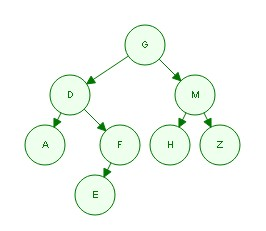
\includegraphics[scale = 1]{Tree_Mid_First.jpg}
					\caption{根据先序和中序确定二叉树}
					\label{mid_first}
				\end{figure}
		
		\subparagraph{四、代码实现思路}


	\subsection{平衡二叉树}
		我们知道,对于一般的二叉搜索树(Binary Search Tree),其期望高度(即为一棵平衡树时)为log2n,其各操作的时间复杂度O(log2n)同时也由此而决定。但是,在某些极端的情况下(如在插入的序列是有序的时),二叉搜索树将退化成近似链或链,此时,其操作的时间复杂度将退化成线性的,即O(n)。我们可以通过随机化建立二叉搜索树来尽量的避免这种情况,但是在进行了多次的操作之后,由于在删除时,我们总是选择将待删除节点的后继代替它本身,这样就会造成总是右边的节点数目减少,以至于树向左偏沉。这同时也会造成树的平衡性受到破坏,提高它的操作的时间复杂度。于是就有了我们下边介绍的平衡二叉树。
		
		平衡二叉树定义:平衡二叉树(Balanced Binary Tree)又被称为AVL树(有别于AVL算法),且具有以下性质:它是一 棵空树或\textbf{它的左右两个子树的高度差的绝对值不超过1,并且左右两个子树都是一棵平衡二叉树}。平衡二叉树的常用算法有红黑树、AVL树等。在平衡二叉搜索树中,我们可以看到,\textbf{其高度一般都良好地维持在O(log2n),大大降低了操作的时间复杂度}。
		
		最小二叉平衡树的节点的公式如下:
		
		F(n)=F(n-1)+F(n-2)+1
		
		这个类似于一个递归的数列,可以参考Fibonacci数列,1是根节点,F(n-1)是左子树的节点数量,F(n-2)是右子树的节点数量。
		\begin{lstlisting}
	// 求树高度
	int high(btnode *T)  
	{  
		if(T==NULL)  
			return 0;  
		else  
			return max(high(T->lchild),high(T->rchild))+1;  
	}  
	
	
	// 方法2
	void high(bnode *T,int &h)    引用h为树的高度  
	{  
		if(T==NULL)  
			h=0;  
		else  
		{  
			int h1,h2;  
			high(T->lchild,h1);  
			high(T->rchild,h2);  
			h=max(h1,h2)+1;  
		}  
	}  
		\end{lstlisting}
		
		\subsubsection{平衡查找树之AVL树}
			AVL树定义:AVL树是最先发明的自平衡二叉查找树。在AVL中任何节点的两个儿子子树的高度最大差别为1,所以它也被称为高度平衡树,n个结点的AVL树最大深度约1.44log2n。查找、插入和删除在平均和最坏情况下都是O(logn)。增加和删除可能需要通过一次或多次树旋转来重新平衡这个树。这个方案很好的解决了二叉查找树退化成链表的问题,把插入,查找,删除的时间复杂度最好情况和最坏情况都维持在O(logN)。但是频繁旋转会使插入和删除牺牲掉O(logN)左右的时间,不过相对二叉查找树来说,时间上稳定了很多。
			
			AVL树的自平衡操作——旋转:
			
			AVL树最关键的也是最难的一步操作就是旋转。旋转主要是为了实现AVL树在实施了插入和删除操作以后,树重新回到平衡的方法。下面我们重点研究一下AVL树的旋转。
			
			对于一个平衡的节点,由于任意节点最多有两个儿子,因此高度不平衡时,此节点的两颗子树的高度差2.容易看出,这种不平衡出现在下面四种情况:
			\begin{figure}[h]
				\centering
				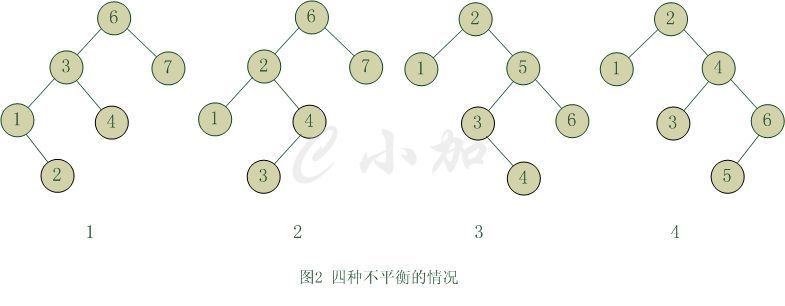
\includegraphics[scale = 0.8]{AVL.jpg}
				\caption{AVL 4种不平衡}
				\label{AVL}
			\end{figure}
				
			\begin{enumerate}[itemindent = 1em,label = (\arabic{enumi})]
				\item  6节点的左子树3节点高度比右子树7节点大2,左子树3节点的左子树1节点高度大于右子树4节点,这种情况成为左左。
				\item  6节点的左子树2节点高度比右子树7节点大2,左子树2节点的左子树1节点高度小于右子树4节点,这种情况成为左右。
				\item  2节点的左子树1节点高度比右子树5节点小2,右子树5节点的左子树3节点高度大于右子树6节点,这种情况成为右左。
				\item  2节点的左子树1节点高度比右子树4节点小2,右子树4节点的左子树3节点高度小于右子树6节点,这种情况成为右右。
			\end{enumerate}
			
			从图\ref{AVL}中可以可以看出,1和4两种情况是对称的,这两种情况的旋转算法是一致的,只需要经过一次旋转就可以达到目标,我们称之为单旋转。2和3两种情况也是对称的,这两种情况的旋转算法也是一致的,需要进行两次旋转,我们称之为双旋转。
				
			\subparagraph{单旋转}:
			
				单旋转是针对于\textbf{左左}和\textbf{右右}这两种情况的解决方案,这两种情况是对称的,只要解决了左左这种情况,右右就很好办了。图3是左左情况的解决方案,节点k2不满足平衡特性,因为它的左子树k1比右子树Z深2层,而且k1子树中,更深的一层的是k1的左子树X子树,所以属于左左情况。
					\begin{figure}[h]
						\centering
						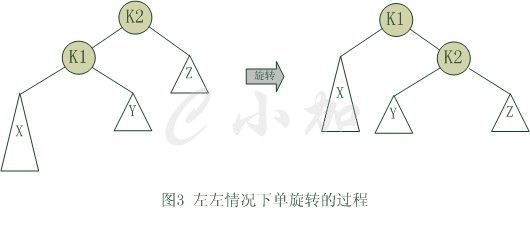
\includegraphics[scale = 0.8]{Rotate_1.jpg}
						\caption{AVL 单旋转}
					\end{figure}
					
				为使树恢复平衡,我们把k2变成这棵树的根节点,因为k2大于k1,把k2置于k1的右子树上,而原本在k1右子树的Y大于k1,小于k2,就把Y置于k2的左子树上,这样既满足了二叉查找树的性质,又满足了平衡二叉树的性质。
				
				这样的操作只需要一部分指针改变,结果我们得到另外一颗二叉查找树,它是一棵AVL树,因为X向上一移动了一层,Y还停留在原来的层面上,Z向下移动了一层。整棵树的新高度和之前没有在左子树上插入的高度相同,插入操作使得X高度长高了。因此,由于这颗子树高度没有变化,所以通往根节点的路径就不需要继续旋转了。
					
			\subparagraph{双旋转}:
			
				对于\textbf{左右}和\textbf{右左}这两种情况,单旋转不能使它达到一个平衡状态,要经过两次旋转。双旋转是针对于这两种情况的解决方案,同样的,这样两种情况也是对称的,只要解决了左右这种情况,右左就很好办了。图4是左右情况的解决方案,节点k3不满足平衡特性,因为它的左子树k1比右子树Z深2层,而且k1子树中,更深的一层的是k1的右子树k2子树,所以属于左右情况。
				\begin{figure}[h]
					\centering
					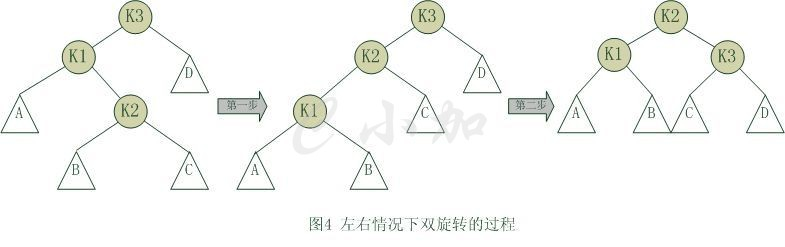
\includegraphics[scale = 0.8]{Rotate_2.jpg}
					\caption{AVL 双旋转}
				\end{figure}
				
				为使树恢复平衡,我们需要进行两步,第一步,把k1作为根,进行一次右右旋转,旋转之后就变成了左左情况,所以第二步再进行一次左左旋转,最后得到了一棵以k2为根的平衡二叉树。
			
			\subparagraph{实现}:
			\begin{lstlisting}
//AVL树节点信息
template<class T>
class TreeNode
{
public:
	TreeNode():lson(NULL),rson(NULL),freq(1),hgt(0){}
	T data;//值
	int hgt;//高度
	unsigned int freq;//频率
	TreeNode* lson;//指向左儿子的地址
	TreeNode* rson;//指向右儿子的地址
};

//AVL树类的属性和方法声明
template<class T>
class AVLTree
{
private:
	TreeNode<T>* root;//根节点
	void insertpri(TreeNode<T>* &node,T x);//插入
	TreeNode<T>* findpri(TreeNode<T>* node,T x);//查找
	void insubtree(TreeNode<T>* node);//中序遍历
	void Deletepri(TreeNode<T>* &node,T x);//删除
	int height(TreeNode<T>* node);//求树的高度
	void SingRotateLeft(TreeNode<T>* &k2);//左左情况下的旋转
	void SingRotateRight(TreeNode<T>* &k2);//右右情况下的旋转
	void DoubleRotateLR(TreeNode<T>* &k3);//左右情况下的旋转
	void DoubleRotateRL(TreeNode<T>* &k3);//右左情况下的旋转
	int Max(int cmpa,int cmpb);//求最大值

public:
	AVLTree():root(NULL){}
	void insert(T x);//插入接口
	TreeNode<T>* find(T x);//查找接口
	void Delete(T x);//删除接口
	void traversal();//遍历接口

};
//计算节点的高度
template<class T>
int AVLTree<T>::height(TreeNode<T>* node)
{
	if(node!=NULL)
		return node->hgt;
	return -1;
}
//求最大值
template<class T>
int AVLTree<T>::Max(int cmpa,int cmpb)
{
	return cmpa>cmpb?cmpa:cmpb;
}
//左左情况下的旋转
template<class T>
void AVLTree<T>::SingRotateLeft(TreeNode<T>* &k2)
{
	TreeNode<T>* k1;
	k1=k2->lson;
	k2->lson=k1->rson;
	k1->rson=k2;
	
	k2->hgt=Max(height(k2->lson),height(k2->rson))+1;
	k1->hgt=Max(height(k1->lson),k2->hgt)+1;
}
//右右情况下的旋转
template<class T>
void AVLTree<T>::SingRotateRight(TreeNode<T>* &k2)
{
	TreeNode<T>* k1;
	k1=k2->rson;
	k2->rson=k1->lson;
	k1->lson=k2;
	
	k2->hgt=Max(height(k2->lson),height(k2->rson))+1;
	k1->hgt=Max(height(k1->rson),k2->hgt)+1;
}
//左右情况的旋转
template<class T>
void AVLTree<T>::DoubleRotateLR(TreeNode<T>* &k3)
{
	SingRotateRight(k3->lson);
	SingRotateLeft(k3);
}
//右左情况的旋转
template<class T>
void AVLTree<T>::DoubleRotateRL(TreeNode<T>* &k3)
{
	SingRotateLeft(k3->rson);
	SingRotateRight(k3);
}
//插入
template<class T>
void AVLTree<T>::insertpri(TreeNode<T>* &node,T x)
{
	if(node==NULL)//如果节点为空,就在此节点处加入x信息
	{
		node=new TreeNode<T>();
		node->data=x;
		return;
	}
	if(node->data>x)//如果x小于节点的值,就继续在节点的左子树中插入x
	{
		insertpri(node->lson,x);
		if(2==height(node->lson)-height(node->rson))
			if(x<node->lson->data)
				SingRotateLeft(node);
			else
				DoubleRotateLR(node);
	}
	else if(node->data<x)//如果x大于节点的值,就继续在节点的右子树中插入x
	{
		insertpri(node->rson,x);
		if(2==height(node->rson)-height(node->lson))//如果高度之差为2的话就失去了平衡,需要旋转
			if(x>node->rson->data)
				SingRotateRight(node);
			else
				DoubleRotateRL(node);
	}
	else ++(node->freq);//如果相等,就把频率加1
	node->hgt=Max(height(node->lson),height(node->rson));
}
//插入接口
template<class T>
void AVLTree<T>::insert(T x)
{
	insertpri(root,x);
}
//查找
template<class T>
TreeNode<T>* AVLTree<T>::findpri(TreeNode<T>* node,T x)
{
	if(node==NULL)//如果节点为空说明没找到,返回NULL
	{
		return NULL;
	}
	if(node->data>x)//如果x小于节点的值,就继续在节点的左子树中查找x
	{
		return findpri(node->lson,x);
	}
	else if(node->data<x)//如果x大于节点的值,就继续在节点的左子树中查找x
	{
		return findpri(node->rson,x);
	}
	else return node;//如果相等,就找到了此节点
}
//查找接口
template<class T>
TreeNode<T>* AVLTree<T>::find(T x)
{
	return findpri(root,x);
}
//删除
template<class T>
void AVLTree<T>::Deletepri(TreeNode<T>* &node,T x)
{
	if(node==NULL) return ;//没有找到值是x的节点
	if(x < node->data)
	{
		Deletepri(node->lson,x);//如果x小于节点的值,就继续在节点的左子树中删除x
		if(2==height(node->rson)-height(node->lson))
			if(node->rson->lson!=NULL&&(height(node->rson->lson)>height(node->rson->rson)) )
				DoubleRotateRL(node);
			else
				SingRotateRight(node);
	}
	
	else if(x > node->data)
	{
		Deletepri(node->rson,x);//如果x大于节点的值,就继续在节点的右子树中删除x
		if(2==height(node->lson)-height(node->rson))
			if(node->lson->rson!=NULL&& (height(node->lson->rson)>height(node->lson->lson) ))
				DoubleRotateLR(node);
			else
				SingRotateLeft(node);
	}
	
	else//如果相等,此节点就是要删除的节点
	{
		if(node->lson&&node->rson)//此节点有两个儿子
		{
			TreeNode<T>* temp=node->rson;//temp指向节点的右儿子
			while(temp->lson!=NULL) temp=temp->lson;//找到右子树中值最小的节点
			//把右子树中最小节点的值赋值给本节点
			node->data=temp->data;
			node->freq=temp->freq;
			Deletepri(node->rson,temp->data);//删除右子树中最小值的节点
			if(2==height(node->lson)-height(node->rson))
			{
				if(node->lson->rson!=NULL&& (height(node->lson->rson)>height(node->lson->lson) ))
				DoubleRotateLR(node);
				else
				SingRotateLeft(node);
			}
		}
		else//此节点有1个或0个儿子
		{
			TreeNode<T>* temp=node;
			if(node->lson==NULL)//有右儿子或者没有儿子
				node=node->rson;
			else if(node->rson==NULL)//有左儿子
				node=node->lson;
			delete(temp);
			temp=NULL;
		}
	}
	
	if(node==NULL) return;
	node->hgt=Max(height(node->lson),height(node->rson))+1;
	return;
}
//删除接口
template<class T>
void AVLTree<T>::Delete(T x)
{
	Deletepri(root,x);
}
//中序遍历函数
template<class T>
void AVLTree<T>::insubtree(TreeNode<T>* node)
{
	if(node==NULL) return;
	insubtree(node->lson);//先遍历左子树
	cout<<node->data<<" ";//输出根节点
	insubtree(node->rson);//再遍历右子树
}
//中序遍历接口
template<class T>
void AVLTree<T>::traversal()
{
	insubtree(root);
}
			\end{lstlisting}
		\subsubsection{平衡查找树之红黑树}
			红黑树的\textbf{定义}:红黑树是一种自平衡二叉查找树,是在计算机科学中用到的一种数据结构,典型的用途是实现关联数组。它是在1972年由鲁道夫·贝尔发明的,称之为"对称二叉B树",它现代的名字是在 Leo J. Guibas 和 Robert Sedgewick 于1978年写的一篇论文中获得的。它是复杂的,但它的操作有着良好的最坏情况运行时间,并且在实践中是高效的: 它可以在O(logn)时间内做查找,插入和删除,这里的n是树中元素的数目。
			
			红黑树和AVL树一样都对插入时间、删除时间和查找时间提供了最好可能的最坏情况担保。这不只是使它们在时间敏感的应用如实时应用(real time application)中有价值,而且使它们有在提供最坏情况担保的其他数据结构中作为建造板块的价值;例如,在计算几何中使用的很多数据结构都可以基于红黑树。此外,红黑树还是2-3-4树的一种等同,它们的思想是一样的,只不过红黑树是2-3-4树用二叉树的形式表示的。
			
			\subparagraph{红黑树的性质}:
			
				红黑树是每个节点都带有颜色属性的二叉查找树,颜色为红色或黑色。在二叉查找树强制的一般要求以外,对于任何有效的红黑树我们增加了如下的额外要求:
				
				性质1. 节点是红色或黑色。
				
				性质2. 根是黑色。
				
				性质3. 所有叶子都是黑色(叶子是NIL节点)。
				
				性质4. 每个红色节点必须有两个黑色的子节点。(从每个叶子到根的所有路径上不能有两个连续的红色节点。)
				
				性质5. 从任一节点到其每个叶子的所有简单路径都包含相同数目的黑色节点。
		\subsubsection{B 树}
			B树也是一种用于查找的平衡树,但是它不是二叉树。
			
			B树的定义:B树(B-tree)是一种树状数据结构,能够用来存储排序后的数据。这种数据结构能够让查找数据、循序存取、插入数据及删除的动作,都在对数时间内完成。B树,概括来说是一个一般化的二叉查找树,可以拥有多于2个子节点。与自平衡二叉查找树不同,B-树为系统最优化大块数据的读和写操作。B-tree算法减少定位记录时所经历的中间过程,从而加快存取速度。这种数据结构常被应用在数据库和文件系统的实作上。
			
			在B树中查找给定关键字的方法是,首先把根结点取来,在根结点所包含的关键字K1,…,Kn查找给定的关键字(可用顺序查找或二分查找法),若找到等于给定值的关键字,则查找成功;否则,一定可以确定要查找的关键字在Ki与Ki+1之间,Pi为指向子树根节点的指针,此时取指针Pi所指的结点继续查找,直至找到,或指针Pi为空时查找失败。
			
			B树作为一种多路搜索树(并不是二叉的):
			
			1) 定义任意非叶子结点最多只有M个儿子;且M>2;
			
			2) 根结点的儿子数为[2, M];
			
			3) 除根结点以外的非叶子结点的儿子数为[M/2, M];
			
			4) 每个结点存放至少M/2-1(取上整)和至多M-1个关键字;(至少2个关键字)
			
			5) 非叶子结点的关键字个数=指向儿子的指针个数-1;
			
			6) 非叶子结点的关键字:K[1], K[2], …, K[M-1];且K[i] < K[i+1];
			
			7) 非叶子结点的指针:P[1], P[2], …, P[M];其中P[1]指向关键字小于K[1]的子树,P[M]指向关键字大于K[M-1]的子树,其它P[i]指向关键字属于(K[i-1], K[i])的子树;
			
			8) 所有叶子结点位于同一层;
		
		\subsubsection{B+ 树}
			B+树是B树的变体,也是一种多路搜索树:
			
			1) 其定义基本与B-树相同,除了:
			
			2) 非叶子结点的子树指针与关键字个数相同;
			
			3) 非叶子结点的子树指针P[i],指向关键字值属于[K[i], K[i+1])的子树(B-树是开区间);
			
			4) 为所有叶子结点增加一个链指针;
			
			5) 所有关键字都在叶子结点出现;
			
		\subsubsection{B* 树}
			B*树是B+树的变体,在B+树的非根和非叶子结点再增加指向兄弟的指针,将结点的最低利用率从1/2提高到2/3。
		
	\subsection{Trie 字典树}	
		Tire树称为字典树,又称单词查找树,Trie树,是一种树形结构,是一种哈希树的变种。典型应用是用于统计,排序和保存大量的字符串(但不仅限于字符串),所以经常被搜索引擎系统用于文本词频统计。它的优点是:利用字符串的公共前缀来减少查询时间,最大限度地减少无谓的字符串比较,查询效率比哈希树高。 
		
		Tire树的三个基本性质:
		
		1) 根节点不包含字符,除根节点外每一个节点都只包含一个字符; 
		
		2) 从根节点到某一节点,路径上经过的字符连接起来,为该节点对应的字符串; 
		
		3) 每个节点的所有子节点包含的字符都不相同。
		
		Tire树的应用:
		
		1) 串的快速检索
		
		给出N个单词组成的熟词表,以及一篇全用小写英文书写的文章,请你按最早出现的顺序写出所有不在熟词表中的生词。
		
		在这道题中,我们可以用数组枚举,用哈希,用字典树,先把熟词建一棵树,然后读入文章进行比较,这种方法效率是比较高的。
		
		2) “串”排序
		
		给定N个互不相同的仅由一个单词构成的英文名,让你将他们按字典序从小到大输出。用字典树进行排序,采用数组的方式创建字典树,这棵树的每个结点的所有儿子很显然地按照其字母大小排序。对这棵树进行先序遍历即可。
		
		3) 最长公共前缀
		
		对所有串建立字典树,对于两个串的最长公共前缀的长度即他们所在的结点的公共祖先个数,于是,问题就转化为求公共祖先的问题。

\newpage
\section{priority\_queue<int, vector<int>, greater<int> >}
	\subsection{特点}
		\begin{itemize}
			\item 允许重复元素
			\item 一种适配器[包装了底层容器如vector 的 高层抽象]
			\item 可(pop())、(push())
			\item pop() 的元素永远为当前序列里中最小或最大的。
		\end{itemize}
	\subsection{用途}


\newpage
\section{Vector}
	\subsection{关于内存泄露的检验}
		随着用string越来越多,有的时候你会发现string的内存管理的问题,存在内存暂时泄露的问题。这个内存泄露与我们常规说的内存泄露问题不一样。\textbf{它不是真的内存泄露,在程序结束的时候,内存还是会释放掉的,但是在程序的运行过程中,内存被string or  vector对象占用着}。比如你有个string对象保存了一个比较大的网页,用完了之后,你想通过clear来回收这个对象的内存,你这样是做不到的。因为string的clear并不会真正回收string对象分配内存。那要怎么做才能做到呢?
		
		vector 与 string 类似,而string比较少。
		\begin{lstlisting}
	vector<int> test;
	
	cout << test.capacity() << endl;
	cout << "after pushOneData test capacity is " << test.capacity() << endl;
	
	for (int i = 0; i < 100; ++i)
	test.push_back(i);
	
	cout << "after pushSomeData test capacity is " << test.capacity() << endl;
	
	test.clear();
	
	cout << "after clear test capacity is " << test.capacity() << endl;
	
	test.shrink_to_fit();
	//test.swap(vector<int>()); 同样可以解决内存泄露问题.. 交换一个空的临时对象.. 这样就可以利用对象在离开作用域时析构的特性了
	
	
	cout << "after shrink_to_fit test capacity is " << test.capacity() << endl;
		\end{lstlisting}

		\begin{figure}[h]
			\centering
			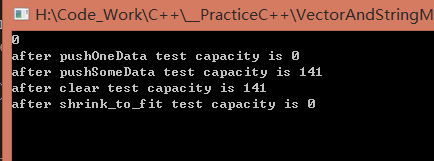
\includegraphics[scale = 1]{VectorMemoryleak.png}
			\caption{vector 内存泄露检测}
		\end{figure}
		
		\subparagraph{Notice}vector依旧string clear后,需要调用.shrink\_to\_fit 才可将内存清除,防止内存泄露,或者与一个同类型空容器交换以释放内存。
	\subsection{细节}
		\subsubsection{push\_back 与 emplace\_back} \url{http://blog.csdn.net/yockie/article/details/52674366}	
		\begin{lstlisting}
	#include <vector>
	#include <string>
	#include "time_interval.h"
	
	class Foo {
	public:
		Foo(std::string str) : name(str) {
			std::cout << "constructor" << std::endl;
		}
		Foo(const Foo& f) : name(f.name) {
			std::cout << "copy constructor" << std::endl;
		}
		Foo(Foo&& f) : name(std::move(f.name)){
			std::cout << "move constructor" << std::endl;
		}
		
	private:
		std::string name;
	};
	int main() 
	{
		std::vector<Foo> v;
		int count = 10000000;
		v.reserve(count);       //预分配十万大小,排除掉分配内存的时间
		
		{
			TIME_INTERVAL_SCOPE("push_back T:");
			Foo temp("ceshi");
			v.push_back(temp);// push_back(const T&),参数是左值引用
			//打印结果:
			//constructor
			//copy constructor
		}
		
		v.clear();
		{
			TIME_INTERVAL_SCOPE("push_back move(T):");
			Foo temp("ceshi");
			v.push_back(std::move(temp));// push_back(T &&), 参数是右值引用
			//打印结果:
			//constructor
			//move constructor
		}
		
		v.clear();
		{
			TIME_INTERVAL_SCOPE("push_back(T&&):");
			v.push_back(Foo("ceshi"));// push_back(T &&), 参数是右值引用
			//打印结果:
			//constructor
			//move constructor
		}
		
		v.clear();
		{
			std::string temp = "ceshi";
			TIME_INTERVAL_SCOPE("push_back(string):");
			v.push_back(temp);// push_back(T &&), 参数是右值引用
			//打印结果:
			//constructor
			//move constructor
		}
		
		v.clear();
		{
			std::string temp = "ceshi";
			TIME_INTERVAL_SCOPE("emplace_back(string):");
			v.emplace_back(temp);// 只有一次构造函数,不调用拷贝构造函数,速度最快
			//打印结果:
			//constructor
		}
	}
		\end{lstlisting}	
\newpage
\section{List}
	\subsection{特点}
		\begin{itemize}
			\item 允许重复元素
			\item 实现了基本的 == 和 != 等(如果两个链表里的元素都相等返回true)
			\item 底层数据结构为 双向链表
			\item 可前(push\_front())、后(push\_back())、任意位置插入(insert())
			\item 当然就有pop了
		\end{itemize}
	\subsection{用途}
		
\newpage
\section{Set }
	\subsection{排序}http://blog.csdn.net/wangran51/article/details/8836160
	
	\subsection{特点}
		\begin{itemize}
			\item 无重复元素
			\item 元素默认升序排序【1,2,3】
			\item 高效的查找:红黑二叉检索树
			\item 不可以修改元素
			\item 快捷的删除
		\end{itemize}
	\subsection{用途}
		主要用于检索数据



\newpage
\section{Map}	
 	\subsection{特点}
	 	\begin{itemize}
	 		\item 无重复元素
	 		\item 高效的查找:红黑二叉检索树,查找和添加的复杂度都为O(log(n)),unordered\_map 使用hash表作为基本的存储结构,O(1)。
	 		\item 可以修改元素
	 		\item 快捷的删除
	 	\end{itemize} 
	 \subsection{使用}
		\subsubsection{map最基本的构造函数} 
			\begin{itemize}
				\item  map<string , int >mapstring;
				\item  map< char ,string>mapchar;
				\item  map<int ,char >mapint;
			\end{itemize}
		\subsubsection{map添加数据}
			\begin{itemize}
				\item map<int ,string> maplive;
			\end{itemize}
			\begin{enumerate}
				\item maplive.insert(pair<int,string>(102,"aclive"));
				\item maplive.insert(map<int,string>::value\_type(321,"hai"));
				\item maplive[112]="April";    map中最简单最常用的插入添加!
			\end{enumerate}
		\subsubsection{map中元素的查找}
			\begin{itemize}
				\item 定义迭代器 准备保存 查找返回位置:map<int ,string >::iterator l\_it;
				\item Find 函数: l\_it=maplive.find(112);
				\item 结果判断: if(l\_it==maplive.end()) not find
			\end{itemize}
		\subsubsection{map中元素的删除}
			先查找,返回迭代器位置,erase.
			
		\subsubsection{map的sort问题} 
			Map中的元素是自动按key升序排序,所以不能对map用sort函数 
		
		\subsubsection{其他操作函数}
			\begin{itemize}
				\item begin()          返回指向map头部的迭代器
				\item clear()         删除所有元素
				\item count()          返回指定元素出现的次数
				\item rbegin()         返回一个指向map尾部的逆向迭代器
				\item size()           返回map中元素的个数
			\end{itemize}
	 	
	 	
\newpage
\section{Hash序列--> unordered\_map or set}	
	\subsection{特点}
		\begin{itemize}
			\item 无重复元素
			\item 高效的查找:查找和添加复杂度均为O(1)
			\item 可以修改元素
			\item 快捷的删除
		\end{itemize}
	\subsection{Hash tables}
		Including hash tables (unordered associative containers) in the C++ standard library is one of the most recurring requests. It was not adopted in C++03 due to time constraints only. Although hash tables are less efficient than a balanced tree in the worst case (in the presence of many collisions), they perform better in many real applications.
		
		Collisions are managed only via linear chaining because the committee didn't consider it to be opportune to standardize solutions of open addressing that introduce quite a lot of intrinsic problems (above all when erasure of elements is admitted). To avoid name clashes with non-standard libraries that developed their own hash table implementations, the prefix \textbf{“unordered”} was used \textit{instead of} \textbf{“hash”}.
		
		The new library has four types of hash tables, differentiated by whether or not they accept elements with the same key (\textbf{unique keys or equivalent keys}), and whether they map each key to an associated value. They correspond to the four existing binary-search-tree-based associative containers, with an unordered\_ prefix.
		
		\begin{figure}[h]
			\centering
			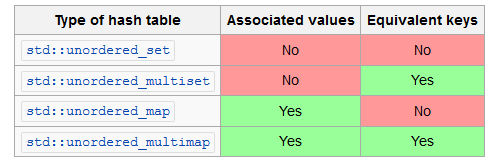
\includegraphics[width = 15cm]{Hash_Table.png}
			\caption{HashTable - 4types}
		\end{figure}
		
	\begin{lstlisting}
		#include <iostream>
		#include <string>
		#include <unordered_map>
		
		int main()
		{
			std::unordered_map<std::string, int> months;
			months["january"] = 31;
			months["february"] = 28;
			months["march"] = 31;
			months["april"] = 30;
			months["may"] = 31;
			months["june"] = 30;
			months["july"] = 31;
			months["august"] = 31;
			months["september"] = 30;
			months["october"] = 31;
			months["november"] = 30;
			months["december"] = 31;
			std::cout << "september -> " << months["september"] << std::endl;
			std::cout << "april     -> " << months["april"] << std::endl;
			std::cout << "december  -> " << months["december"] << std::endl;
			std::cout << "february  -> " << months["february"] << std::endl;
			return 0;
		}
	\end{lstlisting}
	\subsection{实现}
		HashMap基于hash table(哈希表)。 哈希表最大的优点,就是把数据的存储和查找消耗的时间大大降低,几乎可以看成是常数时间;而代价仅仅是消耗比较多的内存。然而在当前可利用内存越来越多的情况下,用空间换时间的做法是值得的 
		
		其基本原理是:使用一个下标范围比较大的数组来存储元素。可以设计一个函数(哈希函数,也叫做散列函数),使得每个元素的关键字都与一个函数值(即数组下标,hash值)相对应,于是用这个数组单元来存储这个元素;也可以简单的理解为,按照关键字为每一个元素“分类”,然后将这个元素存储在相应“类”所对应的地方,称为桶。
		
		但是,不能够保证每个元素的关键字与函数值是一一对应的,因此极有可能出现对于不同的元素,却计算出了相同的函数值,这样就产生了“冲突”,换句话说,就是把不同的元素分在了相同的“类”之中。 总的来说,“直接定址”与“解决冲突”是哈希表的两大特点  
		
		HashMap,首先分配一大片内存,形成许多桶。是利用hash函数,对key进行映射到不同区域(桶)进行保存。
		
		\textbf{插入过程是}:
			\begin{enumerate}[itemindent = 1em]
				\item 得到key
				\item 通过hash函数得到hash值
				\item 得到桶号(一般都为hash值对桶数求模)
				\item 存放key和value在桶内
			\end{enumerate}
		
		\textbf{取值过程是}:
			\begin{enumerate}[itemindent = 1em]
				\item 得到key
				\item 通过hash函数得到hash值
				\item 得到桶号(一般都为hash值对桶数求模)
				\item 比较桶的内部元素是否与key相等,若都不相等,则没有找到。
				\item 取出相等的记录的value。
			\end{enumerate}
	\subsection{用法}
		与 map 大体一致。


\chapter{迭代器-Iterator}
	\section{性质}
		\begin{itemize}
			\item 它是一个访问容器对象的\textbf{技术手段},通过迭代器可以访问容器中的对象
			\item 功能类似于指针 \textbf{或者}  数组下标,通过指针加减 与 数组下标运算获得下一数据成员

			\item 在实现上,迭代器可以是指针,但并不必须是指针,也不必总是使用数据对象的地址。只要能够访问到数据对象就可以了。
		\end{itemize}
	
	

	\section{使用方法}
		\begin{itemize}
			\item 声明迭代器变量
			
			\item 使用引领操作符访问迭代器指向的当前目标对象
			
			\item 使用\textbf{递增操作符}获得下一对象的访问权
			
			\item 若迭代器新值超出容器的元素范围,\textbf{类似指针值变成NULL,目标对象不可引用}
		\end{itemize}
		
		\begin{lstlisting}
	// 声明如下:
	vector<T>::iterator it;
	list<T>::iterator it;
	deque<T>::iterator it;
	
	#include <iostream>
	#include <algorithm>
	using namespace std;
	const int size = 16;
	int main()
	{
		  int a[size];
		  for( int i = 0; i < size; ++i )  a[i] = i;
		  int key = 7;
		  int * ip = find( a, a + size, key );
		  if( ip == a + size )    //  不要使用NULL做指针测试,直接使用过尾值 [)
			    cout << key << " not found." << endl;
		  else
			    cout << key << " found." << endl;
		  return 0;
	}
	
		\end{lstlisting}
		
	\section{类别}
		\begin{table}[H]
			\centering
			\caption{迭代器类别}
			\begin{tabular}{c|m{15cm}}
				\hline 
				类别 & 功能与使用\\
				\hline
				输入	& 从容器中读取元素\\
				输出  & 向容器中写入元素\\
				正向  & 组合输入迭代器和输出迭代器的功能,并保留在容器中的位置\\
				双向  & 组合正向迭代器和逆向迭代器的功能,支持多遍算法\\
				随机  & 组合双向迭代器的功能与直接访问容器中任何元素的功能,即可向前向后跳过任意个元素\\
				\hline
				\end{tabular}
			\end{table}	
			
			\begin{table}[h]
				\centering
				\caption{不同迭代器对应的可执行操作}
				\begin{tabular}{c|m{15cm}}
					\hline 
					类别 & 可使用的操作\\
					\hline
					所有  & ++p,p++ [位置自增运算]\\
					\hline
					输入  & *p[作为右值], p = q[将一个迭代器赋给另一个迭代器], p == q[相等比较运算,但不能比较大小]\\
					\hline
					输出  & *p[作为左值], p = q[将一个迭代器赋给另一个迭代器]\\
					\hline
					正向  & 提供输入输出迭代器的所有功能\\
					\hline
					双向  & --p,p-- [位置自减运算]\\
					\hline
					随机  & p+=i[将迭代器递增i位],p+i[在p位加i位后的迭代器],p[i][返回p位元素偏离i位的元素引用],p<p1[如果迭代器p的位置在p1前,返回true,否则返回false]\\
					\hline
				\end{tabular}
			\end{table}
			
			\begin{table}[h]
				\centering
				\caption{各容器对应的迭代器类别}
				\begin{tabular}{c|m{15cm}}
					\hline 
					容器类别 & 可使用的迭代器\\
					\hline
					vector	& 随机\\
					deque   & 随机\\
					\hline
					list    & 双向\\
					set     & 双向 multi同\\
					map     & 双向 multi同\\
					\hline
					stack   & 不支持\\
					queue   & 不支持\\
					priority\_queue    & 不支持\\
					\hline
				\end{tabular}
			\end{table}
				
	\section{删除}
		vector用到erase的话,那必须用迭代器了,那么以下就要注意了
		\begin{itemize}
			\item 在执行erase后,不可以进行++pos 操作,否则会报错
			\item 在不执行erase时,要进行++pos 进行前进
		\end{itemize}
\begin{lstlisting}

	  for(auto i = 1; i < nums.size(); )
	  {
		  flag = true;
		  if(nums[i-1] == nums[i])
		  {
			  ++size;
			  if(size > 2)
			  {
				  --lenth;
				  nums.erase(pos);    //这块执行pos 的话就不用再移位置了
				  flag = false;
			  }
		  }
		  else
		  {
			  size = 1;
		  }
		  if(flag)					//否则,移位置前进
		  {
			  ++i;
			  ++pos;
		  }
	  }
\end{lstlisting}
		
	\section{Iterator 失效概要}
		Golden Rule是:\textbf{尽量不要使用容器的插入删除操作之前的迭代器}。
		
		对于vector ,deque, list, 一种可行的方式是:
			\begin{lstlisting}
	std::vector<int>::iterator it = my_container.begin();  
	for (it != my_container.end();/**blank*/ ) {  
		if (*it % 2 == 1) {  
			it = my_container.erase(it);  
		}  
		else{  
			it++;  
		}  
	}  			
	
	
	// Method Two --
	 std::vector<int>::iterator it = my_container.begin();  
	 for (it != my_container.end();/**blank*/ ) {  
		 if (*it % 2 == 1) {  
			 my_container.erase(it++);  
		 }  
		 else{  
			 it++;  
		 }  
	 }  
	 /*
		 my_container.erase(it++) 巧妙得在执行erase()之前,it 先自增,指向被删除元素后面的元素,而给erase()传递的是未自增的it迭代器,以定位要删除的元素。
		 如果元素的值为奇数,则删除此元素,it指向下一个元素,如果元素的值为偶数,则检查下一个元素的值。整个迭代过程中迭代器就不会失效了。
	 */
			\end{lstlisting}
			
	\section{Insertion 失效总结}
		\subsection{Sequence containers}
			\begin{itemize}
				\item \verb|vector|: all iterators and references before the point of insertion are unaffected, unless the new container size is greater than the previous capacity (in which case all iterators and references are invalidated)
				\item \verb|deque|: all iterators and references are invalidated, unless the inserted member is at an end (front or back) of the deque (in which case all iterators are invalidated, but references to elements are unaffected)
				\item \verb|list|: all iterators and references unaffected 
				\item \verb|forward_list|: all iterators and references unaffected (applies to \verb|insert_after|) 
				\item \verb|array|: (n/a)
			\end{itemize}
		\subsection{Associative containers}
			\begin{itemize}
				\item \verb|[multi]{set,map}|: all iterators and references unaffected
			\end{itemize}
		\subsection{Unsorted associative containers}
			\begin{itemize}
				\item \verb|unordered_[multi]{set,map}|: \textbf{all iterators invalidated when rehashing occurs}, but references unaffected [23.2.5/8]. Rehashing does not occur if the insertion does not cause the container's size to exceed z * B where z is the maximum load factor and B the current number of buckets.
			\end{itemize}
		
		\subsection{Container adaptors}
			\begin{itemize}
				\item \verb|stack|: inherited from underlying container
				\item \verb|queue|: inherited from underlying container
				\item \verb|priority_queue|: inherited from underlying container
			\end{itemize}
	\section{Eraser 失效总结}
		\subsection{Sequence containers}
			\begin{itemize}
				\item \verb|vector|: every iterator and reference at or after the point of erase is invalidated 
				\item \verb|deque|: erasing the last element invalidates only iterators and references to the erased elements and the past-the-end iterator; erasing the first element invalidates only iterators and references to the erased elements; erasing any other elements invalidates all iterators and references (including the past-the-end iterator)
				\item \verb|list|: only the iterators and references to the erased element is invalidated  
				\item \verb|forward_list|: only the iterators and references to the erased element is invalidated (applies to \verb|erase_after|) 
				\item \verb|array|: (n/a)
			\end{itemize}
		\subsection{Associative containers}
			\begin{itemize}
				\item \verb|[multi]{set,map}|:  only iterators and references to the erased elements are invalidated 
			\end{itemize}
		\subsection{Unsorted associative containers}
			\begin{itemize}
				\item \verb|unordered_[multi]{set,map}|: all iterators invalidated when rehashing occurs, but references unaffected [23.2.5/8]. Rehashing does not occur if the insertion does not cause the container's size to exceed z * B where z is the maximum load factor and B the current number of buckets.
			\end{itemize}
		
		\subsection{Container adaptors}
			\begin{itemize}
				\item \verb|stack|: inherited from underlying container
				\item \verb|queue|: inherited from underlying container
				\item \verb|priority_queue|: inherited from underlying container
			\end{itemize}

	\section{Resizing 失效总结}
		\subsection{Sequence containers}
			\begin{itemize}
				\item \verb|vector|: as per insert/erase 
				\item \verb|deque|: as per insert/erase 
				\item \verb|list|: as per insert/erase   
				\item \verb|forward_list|: as per insert/erase 
				\item \verb|array|: (n/a)
			\end{itemize}
		\subsection{Associative containers}
			\begin{itemize}
				\item \verb|[multi]{set,map}|:  only iterators and references to the erased elements are invalidated 
			\end{itemize}
		\subsection{Unsorted associative containers}
			\begin{itemize}
				\item \verb|unordered_[multi]{set,map}|: all iterators invalidated when rehashing occurs, but references unaffected [23.2.5/8]. Rehashing does not occur if the insertion does not cause the container's size to exceed z * B where z is the maximum load factor and B the current number of buckets.
			\end{itemize}
		
		\subsection{Container adaptors}
			\begin{itemize}
				\item \verb|stack|: inherited from underlying container
				\item \verb|queue|: inherited from underlying container
				\item \verb|priority_queue|: inherited from underlying container
			\end{itemize}
	\section{Note}
		\begin{itemize}
			\item \textbf{Unless otherwise specified} (either explicitly or by defining a function in terms of other functions), invoking a container member function or passing a container as an argument to \textbf{a library function shall not invalidate iterators }to, or change the values of, objects within that container.
			\item \textbf{no swap() function invalidates any references, pointers, or iterators} referring to the elements of the containers being swapped. [ Note: \textbf{The end() iterator} does not refer to any element, so it \textbf{may be invalidated}. —end note ]
			\item Other than the above caveat regarding swap(), it's not clear whether "end" iterators are subject to the above listed per-container rules; you should assume, anyway, that they are
			\item \verb|vector| and all unordered associative containers support \verb|reserve(n)| which guarantees that no automatic resizing will occur at least until the size of the container grows to \verb|n|. Caution should be taken with unordered associative containers because a future proposal will allow the specification of a minimum load factor, which would allow rehashing to occur on \verb|insert| after enough \verb|erase| operations reduce the container size below the minimum; the guarantee should be considered potentially void after an \verb|erase|.
		\end{itemize}
		
	\section{插入迭代器}
		迭代器是一个纯粹抽象概念:任何东西,只要其行为类似迭代器,它就是一个迭代器。\verb|C++|标准库提供了数个预先定义的特殊迭代器,即迭代器适配器(\verb|iterator adapters|)。它们不仅起辅助作用,还能赋予整个迭代器抽象概念更强大的能力。
		
		说明:适配器是使一事物的行为类似于另一事物的行为的一种机制。
		
		插入器是一种迭代器适配器,带有一个容器参数,并\textbf{生成}一个迭代器,\textit{用于}在指定容器中插入元素。通过插入迭代器赋值时,迭代器将会插入一个新元素。\verb|C++|提供了三种插入器,其差别在于插入元素位置不同。
		\begin{enumerate}
			\item \verb|back_inserter|:创建使用\verb|push_back|实现插入的迭代器
			
			\verb|back_inserter|内部调用\verb|push_back|,在容器末尾插入元素。因此,只有在提供有\verb|push_back|成员函数的容器中才能使用。这样的容器有:\verb|vector,deque,list|。元素排列次序和安插次序相同
			\item \verb|front_inserter|:创建使用\verb|push_front|实现插入的迭代器
			
			\verb|front_inserter|内部调用\verb|push_front|,将元素安插于容器最前端。因此,只有在提供有\verb|push_front|成员函数的容器中才能使用。这样的容器有:\verb|deque,list|。元素排列次序和安插次序相反
			\item \verb|insert|:创建使用\verb|insert|实现插入的迭代器
			
			\verb|Inserter|内部调用\verb|insert|,在它的迭代器实参所标明的位置前面插入元素。所有\verb|STL|容器都提供\verb|insert|成员函数,因此这是唯一可用于关联容器上的插入迭代器。元素排列次序和安插次序相同
		\end{enumerate}
		
		\begin{lstlisting}
	#include <iostream>  
	#include <vector>  
	#include <list>  
	#include <iterator>  
	
	using namespace std;  
	
	template<typename T>  
	void PrintElements(T c)  
	{  
		T::const_iterator itr = c.begin();  
		while(itr != c.end())  
		{  
			cout<<*itr++<<" ";  
		}  
	}  
	
	int main()  
	{  
		vector<int> vecSrc;  
		list<int> vecDest;  
		
		for(vector<int>::size_type i=0; i<3; ++i)  
		{  
			vecSrc.push_back(i);  
		} 
		
		/*
			list<int> coll1; 
			vector<int> coll2;
			copy(coll1.begin(), coll1.end(), back_inserter(coll2));
		*/
		copy(vecSrc.begin(),vecSrc.end(),back_insert_iterator<list<int> >(vecDest));  
		PrintElements(vecDest);  
		cout<<endl;  
		
		copy(vecSrc.begin(),vecSrc.end(),front_insert_iterator<list<int> >(vecDest));  
		PrintElements(vecDest);  
		cout<<endl;  
		
		copy(vecSrc.begin(),vecSrc.end(),insert_iterator<list<int> >(vecDest,++vecDest.begin()));  
		PrintElements(vecDest);  
		
		return 0;  
	}  
	
	// 2 0 1 -  2 1 0 -  0 1 2
		\end{lstlisting}
	
	\section{输入输出迭代器}
		标准程序库定义有供输入及输出用的\verb|iostream iterator|类,称为 \verb|istream_iterator| 和 \verb|ostream_iterator|,分别支持单一型别的元素读取和写入	
		
		\begin{enumerate}
			\item \verb|ostream_iterator|:
				\begin{lstlisting}
	// ostream_iterator example
	#include <iostream>     // std::cout
	#include <iterator>     // std::ostream_iterator
	#include <vector>       // std::vector
	#include <algorithm>    // std::copy
	
	int main () {
		std::vector<int> myvector;
		for (int i=1; i<10; ++i) myvector.push_back(i*10);
		
		std::ostream_iterator<int> out_it (std::cout,", ");
		std::copy ( myvector.begin(), myvector.end(), out_it );
		std::unique_copy(myvector.begin(), myvector.end(), out_it);
		return 0;
	}
	
	// 10, 20, 30, 40, 50, 60, 70, 80, 90, 
				\end{lstlisting}
			\item \verb|istream_iterator|:
			\begin{lstlisting}
	// istream_iterator example
	#include <iostream>     // std::cin, std::cout
	#include <iterator>     // std::istream_iterator
	
	int main () {
		double value1, value2;
		std::cout << "Please, insert two values: ";
		
		std::istream_iterator<double> eos;              // end-of-stream iterator
		std::istream_iterator<double> iit (std::cin);   // stdin iterator
		
		if (iit!=eos) value1=*iit;
		
		++iit;
		if (iit!=eos) value2=*iit;
		
		std::cout << value1 << "*" << value2 << "=" << (value1*value2) << '\n';
		
		return 0;
	}
	
	// Please, insert two values: 2 32 2*32=64
			\end{lstlisting}
		\end{enumerate}	
\section{参考}
		\url{http://www.cnblogs.com/dongzhiquan/archive/2011/01/05/1994523.html}
		
			\url{http://www.cnblogs.com/blueoverflow/p/4923523.html}
			
			失效重要:\url{http://stackoverflow.com/questions/6438086/iterator-invalidation-rules}
			
			\url{http://lib.csdn.net/article/cplusplus/28411}
			
			\verb|C++ STL 插入器:|\url{http://www.linuxidc.com/Linux/2015-02/113456.htm}
			
			\url{http://blog.csdn.net/bonchoix/article/details/8062483}
\chapter{仿函数-Function}
	\section{std::function}
		在C++中,可调用实体主要包括函数,函数指针,函数引用,可以隐式转换为函数指定的对象,或者实现了opetator()的对象。C++0x中,新增加了一个std::function对象,std::function对象是\textbf{对C++中现有的可调用实体的一种类型安全的包裹}(我们知道像函数指针这类可调用实体,是类型不安全的).
		std::function object\textbf{最大的用处就是在实现函数回调},使用者需要注意,它不能被用来检查相等或者不相等
		\begin{lstlisting}
	#include<iostream>// std::cout
	#include<functional>// std::function
	
	void func(void)
	{
		std::cout << __FUNCTION__ << std::endl;
	}
	
	class Foo
	{
	public:
		static int foo_func(int a)
		{
			std::cout << __FUNCTION__ << "(" << a << ") ->: ";
			return a;
		}
	};
	
	class Bar
	{
	public:
		int operator() (int a)
		{
			std::cout << __FUNCTION__ << "(" << a << ") ->: ";
			return a;
		}
	};
	
	int main()
	{
		// 绑定普通函数
		std::function<void(void)> fr1 = func;
		fr1();
		
		// 绑定类的静态成员函数
		std::function<int(int)> fr2 = Foo::foo_func;
		std::cout << fr2(100) << std::endl;
		
		// 绑定仿函数
		Bar bar;
		fr2 = bar;
		std::cout << fr2(200) << std::endl;
		
		return 0;
	}
		\end{lstlisting}
	\section{std::bind}
		bind是这样一种机制,它可以预先把指定可调用实体的某些参数绑定到已有的变量,产生一个新的可调 用实体,这种机制在回调函数的使用过程中也颇为有用。
	
		C++11中提供了std::bind,可以说是一种飞跃的提升,bind本身是一种延迟计算的思想,它本身可以绑定普通函数、全局函数、静态函数、类静态函数甚至是类成员函数。
		
		\textbf{std::bind}用来将可调用对象与其参数一起进行绑定。绑定后可以使用\textbf{std::function}进行保存,并延迟到我们需要的时候调用:
			
			\begin{itemize}
				\item bind预先绑定的参数需要传具体的变量或值进去,对于预先绑定的参数,是pass-by-value的
				\item 对于不事先绑定的参数,需要传std::placeholders进去,从\_1开始,依次递增。placeholder是pass-by-reference的
				\item bind的返回值是可调用实体,可以直接赋给std::function对象
				\item 对于绑定的指针、引用类型的参数,使用者需要保证在可调用实体调用之前,这些参数是可用的
			\end{itemize}
		 
		 在绑定部分参数的时候,通过使用\textbf{std::placeholders}来决定空位参数将会是调用发生时的第几个参数。
		\begin{lstlisting}
	#include <iostream>
	#include <functional>
	using namespace std;
	
	int TestFunc(int a, char c, float f)
	{
		cout << a << endl;
		cout << c << endl;
		cout << f << endl;
		
		return a;
	}
	
	int main()
	{
		auto bindFunc1 = bind(TestFunc, std::placeholders::_1, 'A', 100.1);
		bindFunc1(10);
		
		cout << "=================================\n";
		
		auto bindFunc2 = bind(TestFunc, std::placeholders::_2, std::placeholders::_1, 100.1);
		bindFunc2('B', 10);
		
		cout << "=================================\n";
		
		auto bindFunc3 = bind(TestFunc, std::placeholders::_2, std::placeholders::_3, std::placeholders::_1);
		bindFunc3(100.1, 30, 'C');
		
		return 0;
	}	
	\\ Example 2:
	int add1(int i, int j, int k) {  
		return i + j + k;  
	}  
	
	
	class Utils {  
	public:  
		Utils(const char* name) {  
			strcpy(_name, name);  
		}  
		
		void sayHello(const char* name) const {  
			std::cout << _name << " say: hello " << name << std::endl;  
		}  
		
		static int getId() {  
			return 10001;  
		}   
		
		int operator()(int i, int j, int k) const {  
			return i + j + k;  
		}  
		
		private:  
		char _name[32];  
	};  
	
	int main(void) {  
	
		// 绑定全局函数  
		auto add2 = std::bind(add1, std::placeholders::_1, std::placeholders::_2, 10);  
		// 函数add2 = 绑定add1函数,参数1不变,参数2不变,参数3固定为10.  
		std::cout << typeid(add2).name() << std::endl;  
		std::cout << "add2(1,2) = " << add2(1, 2) << std::endl;  
		
		std::cout << "\n---------------------------" << std::endl;  
		
		// 绑定成员函数  
		Utils utils("Vicky");  
		auto sayHello = std::bind(&Utils::sayHello, utils/*调用者*/, std::placeholders::_1/*参数1*/);  
		sayHello("Jack");  
		
		auto sayHelloToLucy = std::bind(&Utils::sayHello, utils/*调用者*/, "Lucy"/*固定参数1*/);  
		sayHelloToLucy();  
		
		// 绑定静态成员函数  
		auto getId = std::bind(&Utils::getId);  
		std::cout << getId() << std::endl;  
		
		std::cout << "\n---------------------------" << std::endl;  
		
		// 绑定operator函数  
		auto add100 = std::bind(&Utils::operator (), utils, std::placeholders::_1, std::placeholders::_2, 100);  
		std::cout << "add100(1, 2) = " << add100(1, 2) << std::endl;  
		
		// 注意:无法使用std::bind()绑定一个重载函数  
		
		return 0;  
	}  		
		\end{lstlisting}
		
		从上面的代码可以看到,bind能够在绑定时候就同时绑定一部分参数,未提供的参数则使用占位符表示,然后在运行时传入实际的参数值。
		
		PS:绑定的参数将会以值传递的方式传递给具体函数,占位符将会以引用传递。
		
		\subparagraph{参考}:
			\url{http://blog.csdn.net/eclipser1987/article/details/24406203}

\chapter{算法-Algorithm}
	算法(Algorithm),是用来操作容器中的数据的模板函数。例如,STL用sort()来对一个vector中的数据进行排序,用find()来搜索一个list中的对象,函数本身与他们操作的数据的结构和类型无关,因此他们可以在从简单数组到高度复杂容器的任何数据结构上使用;
	
	STL算法部分主要由头文件<algorithm>,<numeric>,<functional>组成。要使用STL中的算法函数必须包含头文件<algorithm>,对于数值算法须包含<numeric>.
	\section{查找算法}
	\begin{table}[H]
		\centering
		\caption{查找算法}
		\begin{tabular}{c|m{13cm}}
			\hline 
			函数名 & 功能与使用\\
			\hline
			\textbf{adjacent\_find}	& 在iterator对标识元素范围内,查找一对相邻重复元素,找到则返回指向这对元素的第一个元素的ForwardIterator。否则返回last。\\
			\hline 
			\textbf{binary\_search}  & 在有序序列中查找value,找到返回true。重载的版本实用指定的比较函数对象或函数指针来判断相等\\
			\hline 
			\textbf{count}  & 利用等于操作符,把标志范围内的元素与输入值比较,返回相等元素个数\\
			\hline 
			\textbf{count\_if}  & 利用输入的操作符,对标志范围内的元素进行操作,返回结果为true的个数\\
			\hline 
			\textbf{equal\_range}  & 功能类似equal,返回一对iterator,第一个表示lower\_bound,第二个表示upper\_bound\\
			\hline 
			\textbf{find}	&利用底层元素的等于操作符,对指定范围内的元素与输入值进行比较。当匹配时,结束搜索,返回该元素的一个InputIterator	\\
			\hline 
			\textbf{find\_end}	& 在指定范围内查找"由输入的另外一对iterator标志的第二个序列"的最后一次出现。找到则返回最后一对的第一个ForwardIterator,否则返回输入的"另外一对"的第一个ForwardIterator。重载版本使用用户输入的操作符代替等于操作	\\
			\hline 
			\textbf{find\_first\_of}	&在指定范围内查找"由输入的另外一对iterator标志的第二个序列"中任意一个元素的第一次出现。重载版本中使用了用户自定义操作符	\\
			\hline 
			\textbf{find\_if}	&使用输入的函数代替等于操作符执行find	\\
			\hline 
			\textbf{lower\_bound}	&返回一个ForwardIterator,指向在有序序列范围内的可以插入指定值而不破坏容器顺序的第一个位置。重载函数使用自定义比较操作	\\
			\hline 
			\textbf{upper\_bound}		&返回一个ForwardIterator,指向在有序序列范围内插入value而不破坏容器顺序的最后一个位置,该位置标志一个大于value的值。重载函数使用自定义比较操作	\\
			\hline 
			\textbf{search}	& 给出两个范围,返回一个ForwardIterator,查找成功指向第一个范围内第一次出现子序列(第二个范围)的位置,查找失败指向last1。重载版本使用自定义的比较操作	\\
			\hline 
			\textbf{search\_n}	& 在指定范围内查找val出现n次的子序列。重载版本使用自定义的比较操作\\
			\hline
		\end{tabular}
	\end{table}	
	\section{排序和通用算法}
	\begin{table}[H]
		\centering
		\caption{排序和通用算法}
		\begin{tabular}{c|m{13cm}}
			\hline 
			函数名 & 功能与使用\\
			\hline
			\textbf{inplace\_merge}	& 合并两个有序序列,结果序列覆盖两端范围。重载版本使用输入的操作进行排序\\
			\hline 
			\textbf{merge}  & 合并两个有序序列,存放到另一个序列。重载版本使用自定义的比较\\
			\hline 
			\textbf{nth\_element}  & 将范围内的序列重新排序,使所有小于第n个元素的元素都出现在它前面,而大于它的都出现在后面。重载版本使用自定义的比较操作\\
			\hline 
			\textbf{partial\_sort}  & 对序列做部分排序,被排序元素个数正好可以被放到范围内。重载版本使用自定义的比较操作\\
			\hline 
			\textbf{partial\_sort\_copy}  & 与partial\_sort类似,不过将经过排序的序列复制到另一个容器\\
			\hline 
			\textbf{partition}	&对指定范围内元素重新排序,使用输入的函数,把结果为true的元素放在结果为false的元素之前	\\
			\hline 
			\textbf{random\_shuffle}	& 对指定范围内的元素随机调整次序。重载版本输入一个随机数产生操作	\\
			\hline 
			\textbf{reverse}	&将指定范围内元素重新反序排序	\\
			\hline 
			\textbf{reverse\_copy}	&与reverse类似,不过将结果写入另一个容器	\\
			\hline 
			\textbf{rotate}	&将指定范围内元素移到容器末尾,由middle指向的元素成为容器第一个元素\\
			\hline 
			\textbf{rotate\_copy}		&与rotate类似,不过将结果写入另一个容器	\\
			\hline 
			\textbf{sort}	& 以升序重新排列指定范围内的元素。重载版本使用自定义的比较操作	\\
			\hline 
			\textbf{stable\_sort}	& 与sort类似,不过保留相等元素之间的顺序关系\\
			\hline
			\textbf{stable\_partition}	& 与partition类似,不过不保证保留容器中的相对顺序\\
			\hline
		\end{tabular}
	\end{table}	
	\section{删除和替换算法}
	\begin{table}[H]
		\centering
		\caption{删除和替换算法}
		\begin{tabular}{c|m{13cm}}
			\hline 
			函数名 & 功能与使用\\
			\hline
			\textbf{copy}	& 复制序列\\
			\hline 
			\textbf{copy\_backward}  & 与copy相同,不过元素是以相反顺序被拷贝\\
			\hline 
			\textbf{iter\_swap}  & 交换两个Forward Iterator的值\\
			\hline 
			\textbf{remove}  & 删除指定范围内所有等于指定元素的元素。注意,该函数不是真正删除函数。内置函数不适合使用remove和remove\_if函数\\
			\hline 
			\textbf{remove\_copy}  & 将所有不匹配元素复制到一个制定容器,返回OutputIterator指向被拷贝的末元素的下一个位置\\
			\hline 
			\textbf{remove\_if}	& 删除指定范围内输入操作结果为true的所有元素\\
			\hline 
			\textbf{remove\_copy\_if}	& 将所有不匹配元素拷贝到一个指定容器\\
			\hline 
			\textbf{replace}	& 将指定范围内所有等于vold的元素都用vnew代替\\
			\hline 
			\textbf{replace\_copy}	&与replace类似,不过将结果写入另一个容器\\
			\hline 
			\textbf{replace\_if}	&将指定范围内所有操作结果为true的元素用新值代替\\
			\hline 
			\textbf{replace\_copy\_if}	&与replace\_if,不过将结果写入另一个容器	\\
			\hline 
			\textbf{swap}	& 交换存储在两个对象中的值\\
			\hline 
			\textbf{swap\_range}	& 将指定范围内的元素与另一个序列元素值进行交换\\
			\hline
			\textbf{unique}	& 清除序列中重复元素,和remove类似,它也不能真正删除元素。重载版本使用自定义比较操作\\
			\hline
			\textbf{unique\_copy}	& 与unique类似,不过把结果输出到另一个容器\\
			\hline
		\end{tabular}
	\end{table}
	 实际上,remove\_if() 等并没有删除容器中的任何元素,它没有改变container.end(), 调用remove\_if()后容器元素个数不会改变!!删除元素的工作
	 交给erase()才能真正删除。
	 
	\section{排列组合算法}
	\begin{table}[H]
		\centering
		\caption{排列组合算法}
		\begin{tabular}{c|m{13cm}}
			\hline 
			函数名 & 功能与使用\\
			\hline
			\textbf{next\_permutation}	& 复制序列\\
			\hline 
			\textbf{prev\_permutation} 	& 取出指定范围内的序列并将它重新排序为上一个序列。如果不存在上一个序列则返回false。重载版本使用自定义的比较操作\\
			\hline 
		\end{tabular}
	\end{table}
	
	\section{生成和异变算法}
	\begin{table}[H]
		\centering
		\caption{生成和异变算法}
		\begin{tabular}{c|m{15cm}}
			\hline 
			函数名 & 功能与使用\\
			\hline
			\textbf{fill}	& 将输入值赋给标志范围内的所有元素\\
			\hline 
			\textbf{fill\_n}  & 将输入值赋给first到first+n范围内的所有元素\\
			\hline 
			\textbf{for\_each}  & 用指定函数依次对指定范围内所有元素进行迭代访问,返回所指定的函数类型。该函数\textbf{不得修改序列中的元素}\\
			\hline 
			\textbf{generate}  & 连续调用输入的函数来填充指定的范围\\
			\hline 
			\textbf{generate\_n}  & 与generate函数类似,填充从指定iterator开始的n个元素\\
			\hline 
			\textbf{transform}	& 将输入的操作作用与指定范围内的每个元素,并产生一个新的序列。重载版本将操作作用在一对元素上,另外一个元素来自输入的另外一个序列。结果输出到指定容器\\
			\hline
		\end{tabular}
	\end{table}	

	\section{关系算法}	
	\begin{table}[H]
		\centering
		\caption{关系算法}
		\begin{tabular}{c|m{12cm}}
			\hline 
			函数名 & 功能与使用\\
			\hline
			\textbf{equal}	& 如果两个序列在标志范围内元素都相等,返回true。重载版本使用输入的操作符代替默认的等于操作符\\
			\hline 
			\textbf{includes}  & 判断第一个指定范围内的所有元素是否都被第二个范围包含,使用底层元素的<操作符,成功返回true。重载版本使用用户输入的函数\\
			\hline 
			\textbf{lexicographical\_compare}  & 比较两个序列。重载版本使用用户自定义比较操作\\
			\hline 
			\textbf{max}  & 返回两个元素中较大一个。重载版本使用自定义比较操作\\
			\hline 
			\textbf{max\_element} & 返回一个Forward Iterator,指出序列中最大的元素。重载版本使用自定义比较操作\\
			\hline 
			\textbf{min}	& 返回两个元素中较小一个。重载版本使用自定义比较操作\\
			\hline 
			\textbf{min\_element}	& 返回一个Forward Iterator,指出序列中最小的元素。重载版本使用自定义比较操作\\
			\hline 
			\textbf{mismatch}	& 并行比较两个序列,指出第一个不匹配的位置,返回一对iterator,标志第一个不匹配元素位置。如果都匹配,返回每个容器的last。重载版本使用自定义的比较操作\\
			\hline 
		\end{tabular}
	\end{table}
	
	\section{集合算法}
		\begin{table}[H]
			\centering
			\caption{集合算法}
			\begin{tabular}{c|m{12cm}}
				\hline 
				函数名 & 功能与使用\\
				\hline
				\textbf{set\_union}	& 构造一个有序序列,包含两个序列中所有的不重复元素。重载版本使用自定义的比较操作\\
				\hline 
				\textbf{set\_intersection}  & 构造一个有序序列,其中元素在两个序列中都存在。重载版本使用自定义的比较操作\\
				\hline 
				\textbf{set\_difference}  & 构造一个有序序列,该序列仅保留第一个序列中存在的而第二个中不存在的元素。重载版本使用自定义的比较操作\\
				\hline 
				\textbf{set\_symmetric\_difference}  & 构造一个有序序列,该序列取两个序列的对称差集(并集-交集)\\
				\hline 
			\end{tabular}
		\end{table}
	
	\section{堆算法}
	\begin{table}[H]
		\centering
		\caption{堆算法}
		\begin{tabular}{c|m{15cm}}
			\hline 
			函数名 & 功能与使用\\
			\hline
			\textbf{make\_heap}	& 把指定范围内的元素生成一个堆。重载版本使用自定义比较操作\\
			\hline 
			\textbf{pop\_heap}  & 并不真正把最大元素从堆中弹出,而是重新排序堆。它把first和last-1交换,然后重新生成一个堆。可使用容器的back来访问被"弹出"的元素或者使用pop\_back进行真正的删除。重载版本使用自定义的比较操作\\
			\hline 
			\textbf{push\_heap}  & 假设first到last-1是一个有效堆,要被加入到堆的元素存放在位置last-1,重新生成堆。在指向该函数前,必须先把元素插入容器后。重载版本使用指定的比较操作\\
			\hline 
			\textbf{sort\_heap} & 对指定范围内的序列重新排序,它假设该序列是个有序堆。重载版本使用自定义比较操作\\
			\hline 
		\end{tabular}
	\end{table}
	
	\section{算术算法}
	\begin{table}[H]
		\centering
		\caption{算术算法}
		\begin{tabular}{c|m{13cm}}
			\hline 
			函数名 & 功能与使用\\
			\hline
			\textbf{accumulate}	& iterator对标识的序列段元素之和,加到一个由val指定的初始值上。重载版本不再做加法,而是传进来的二元操作符被应用到元素上\\
			\hline 
			\textbf{partial\_sum}  & 创建一个新序列,其中每个元素值代表指定范围内该位置前所有元素之和。重载版本使用自定义操作代替加法\\
			\hline 
			\textbf{inner\_product}  & 对两个序列做内积(对应元素相乘,再求和)并将内积加到一个输入的初始值上。重载版本使用用户定义的操作\\
			\hline 
			\textbf{adjacent\_difference} & 创建一个新序列,新序列中每个新值代表当前元素与上一个元素的差。重载版本用指定二元操作计算相邻元素的差\\
			\hline 
		\end{tabular}
	\end{table}
\chapter{参考}
	\url{http://www.cnblogs.com/biyeymyhjob/archive/2012/07/22/2603525.html} 
\end{document} 
 		    